\documentclass[bachelor, och, otchet, hidelinks]{SCWorks}
% параметр - тип обучения - одно из значений:
%    spec     - специальность
%    bachelor - бакалавриат (по умолчанию)
%    master   - магистратура
% параметр - форма обучения - одно из значений:
%    och   - очное (по умолчанию)
%    zaoch - заочное
% параметр - тип работы - одно из значений:
%    referat    - реферат
%    coursework - курсовая работа (по умолчанию)
%    diploma    - дипломная работа
%    pract      - отчет по практике
%    pract      - отчет о научно-исследовательской работе
%    autoref    - автореферат выпускной работы
%    assignment - задание на выпускную квалификационную работу
%    review     - отзыв руководителя
%    critique   - рецензия на выпускную работу
% параметр - включение шрифта
%    times    - включение шрифта Times New Roman (если установлен)
%               по умолчанию выключен
\usepackage[T2A]{fontenc}
\usepackage[utf8]{inputenc}
\usepackage{graphicx}

\usepackage[sort,compress]{cite}
\usepackage{amsmath}
\usepackage{amssymb}
\usepackage{amsthm}
\usepackage{fancyvrb}
\usepackage{longtable}
\usepackage{array}
\usepackage[english,russian]{babel}
%\usepackage{minted}
% Используется автором репозитория
%\usemintedstyle{xcode}
% Этот пакет включает в себя аналогичный Times New Roman шрифт.
% Необходим для успешной компиляции для UNIX-систем ввиду отсутствия TNR в нем.
% Можно использовать и для Windows.
\usepackage{tempora}


\usepackage[colorlinks=false]{hyperref}

\graphicspath{{figures/}}

\newcommand{\eqdef}{\stackrel {\rm def}{=}}

\usepackage{stackengine}
\newcommand\xrowht[2][0]{\addstackgap[.5\dimexpr#2\relax]{\vphantom{#1}}}

\newtheorem{lem}{Лемма}

% % При использовании biblatex вместо bibtex
%\usepackage[style=gost-numeric]{biblatex}
%\addbibresource{thesis.bib}

\begin{document}

% Кафедра (в родительном падеже)
\chair{математической кибернетики и компьютерных наук}

% Тема работы
\title{Триггеры}

% Курс
\course{3}

% Группа
\group{331}

% Факультет (в родительном падеже) (по умолчанию "факультета КНиИТ")
%\department{факультета КНиИТ}

% Специальность/направление код - наименование
%\napravlenie{02.03.02 "--- Фундаментальная информатика и информационные технологии}
%\napravlenie{02.03.01 "--- Математическое обеспечение и администрирование информационных систем}
%\napravlenie{09.03.01 "--- Информатика и вычислительная техника}
%\napravlenie{09.03.04 "--- Программная инженерия}
\napravlenie{10.05.01 "--- Компьютерная безопасность}

% Для студентки. Для работы студента следующая команда не нужна.
%\studenttitle{Студентки}

% Фамилия, имя, отчество в родительном падеже
\author{Бородина Артёма Горовича}

% Заведующий кафедрой
\chtitle{доцент, к.\,ф.-м.\,н.} % степень, звание
\chname{С.\,В.\,Миронов}

%Научный руководитель (для реферата преподаватель проверяющий работу)
\satitle{аспирант}%, к.\,ф.-м.\,н.} %должность, степень, звание
\saname{А.\,А.\,Мартышкин}

% Руководитель практики от организации (только для практики,
% для остальных типов работ не используется)
\patitle{к.\,ф.-м.\,н., доцент}
\paname{Д.\,Ю.\,Петров}

% Семестр (только для практики, для остальных
% типов работ не используется)
\term{2}

% Наименование практики (только для практики, для остальных
% типов работ не используется)
\practtype{учебная}

% Продолжительность практики (количество недель) (только для практики,
% для остальных типов работ не используется)
\duration{2}

% Даты начала и окончания практики (только для практики, для остальных
% типов работ не используется)
\practStart{01.07.2016}
\practFinish{14.07.2016}

% Год выполнения отчета
\date{2022}

\maketitle

% Включение нумерации рисунков, формул и таблиц по разделам
% (по умолчанию - нумерация сквозная)
% (допускается оба вида нумерации)
%\secNumbering


\tableofcontents

% Раздел "Обозначения и сокращения". Может отсутствовать в работе
% \abbreviations
% \begin{description}
%     \item ... "--- ...
%     \item ... "--- ...
% \end{description}

% Раздел "Определения". Может отсутствовать в работе
%\definitions

% Раздел "Определения, обозначения и сокращения". Может отсутствовать в работе.
% Если присутствует, то заменяет собой разделы "Обозначения и сокращения" и "Определения"
%\defabbr


% Раздел "Введение"

\intro

\par Целью данной работы служит ознакомление с основными характеристиками интегральных триггеров \textit{RS, D
, T, JK} и их испытание.

\section*{Задание 1.}
\addcontentsline{toc}{section}{Задание 1}

Запустить лабораторный комплекс Labworks и среду МS10. Открыть файл \textbf{32.5.ms10}, размещенный в папке 
\textbf{Circuit Design Suitе 10.0} среды МS10, или собрать на рабочем поле среды MS10 схему для испытания 
\textit{асинхронного RS-триггера} и установить в диалоговых окнах компонентов их параметры или режимы работы. 
\textbf{Скопировать} схему на страницу отчета.

\begin{figure}[h]
	\center{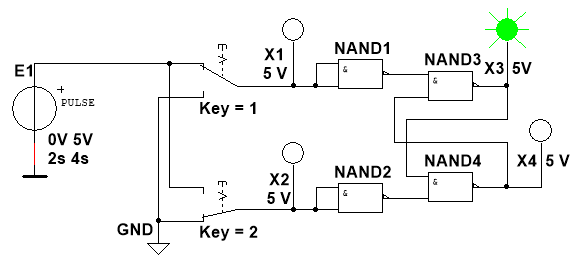
\includegraphics{async_trigger.png}}
	\caption{Схема асинхронного \textit{RS}-триггера.}
\end{figure}

\newpage

Воспользовавшись порядком засвечивания разноцветных пробников и задавая коды (00, 01, 10) состояния ключей 
\textbf{1} и \textbf{2} (входных сигналов), \textbf{составить} таблицу истинности \textit{RS}-триггера. Убедитесь, 
что при запрещенном коде 11 входных сигналов на выходе \textit{RS}-триггера могут засветиться оба пробника, 
или оба не светятся.

\begin{figure}[h]
	\center{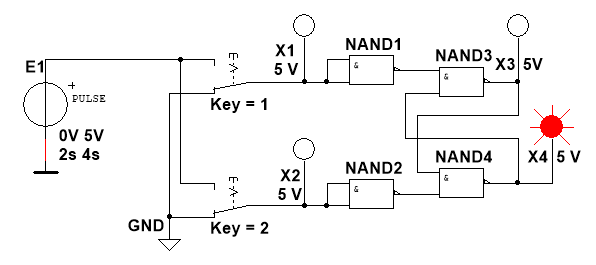
\includegraphics{key_00.png}}
	\caption{Задание кода 00 состояния ключей.}
\end{figure}

\begin{figure}[h]
	\center{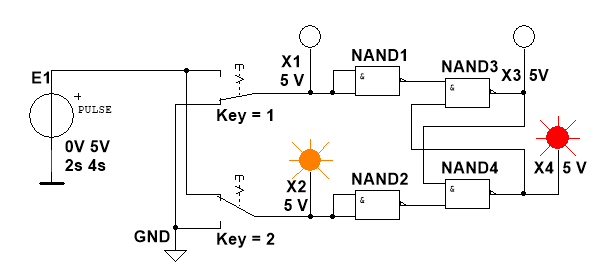
\includegraphics{key_01.png}}
	\caption{Задание кода 01 состояния ключей.}
\end{figure}

\newpage

\begin{figure}[h]
	\center{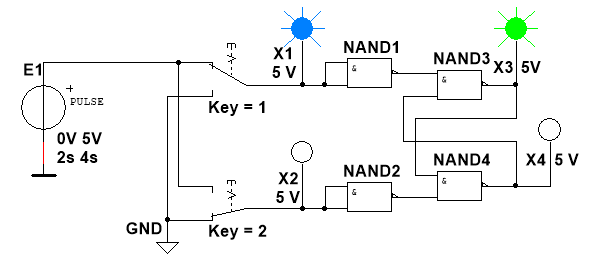
\includegraphics{key_10.png}}
	\caption{Задание кода 10 состояния ключей.}
\end{figure}

\begin{figure}[h]
	\center{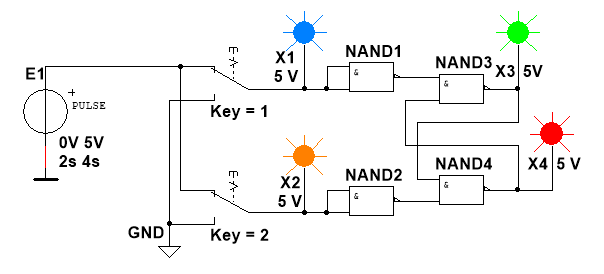
\includegraphics{key_11.png}}
	\caption{Задание кода 11 состояния ключей.}
\end{figure}

Составим таблицу истинности \textit{RS}-триггера.

\begin{table}[h!]
    \centering
	\captionsetup{justification=centering}
	\begin{tabular}{|c|c|c|c|}
		\hline\xrowht[()]{10pt}
		$ S $ & $ R $ & $ Q $ & $ \overline{Q} $ \\
        \hline\xrowht[()]{10pt}
          0   &   0   &   1   &   0   \\
        \hline\xrowht[()]{10pt}
          0   &   1   &   0   &   1   \\
        \hline\xrowht[()]{10pt}
          1   &   0   &   1   &   0   \\
        \hline\xrowht[()]{10pt}
          1   &   1   &   1   &   1   \\
        \hline
	\end{tabular}
	\caption{Таблица истинности \textit{RS}-триггера.}
\end{table}

\newpage

\section*{Задание 2.}
\addcontentsline{toc}{section}{Задание 2}

Подключить к входам триггера логический генератор (генератор слова) \textbf{XWG1}, запрограммировав его первые 
три ячейки кодами 00, 10 и 01 и соединив входы и выходы триггера с входами логического анализатора \textbf{XLA2}.

В диалоговом окне генератора слова \textbf{XWG1 задать} частоту $ f_\text{г} $= 10 кГц и два цикла моделирования 
сигналов (в режиме \textbf{Burst}), а в окне анализатора \textbf{XLA2} – частоту $ f_\text{а} $ = 0,1 МГц таймера, 
уровень высокого напряжения $ U_m $ = 5 В, число импульсов \textbf{Clocks/div} = 8 таймера, приходящихся на одно 
деление.

\textbf{Получить} на экране анализатора \textbf{XLA2} временную диаграмму состояний \textit{RS}-триггера. 
\textbf{Скопировать} схему испытания и временную диаграмму состояния \textit{RS}-триггера на страницу отчета.

\begin{figure}[h]
	\center{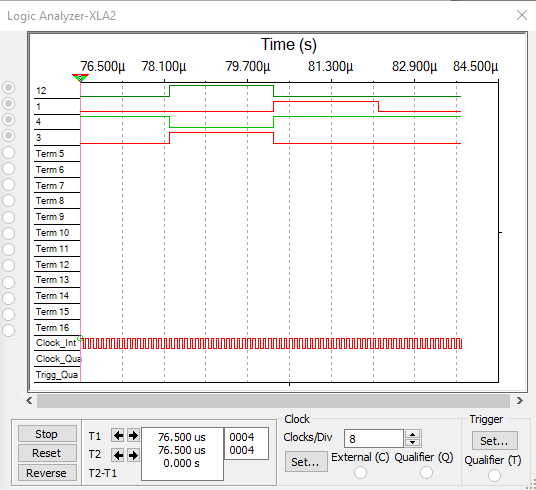
\includegraphics{logic_analyzer.png}}
	\caption{Интерфейс анализатора \textbf{XLA2}.}
\end{figure}

\newpage

\section*{Задание 3.}
\addcontentsline{toc}{section}{Задание 3}

Открыть файл \textbf{32.7.ms10}, размещенный в папке \textbf{Circuit Design Suitе 10.0} среды МS10, или собрать 
на рабочем поле среды MS10 схему для испытания триггеров \textit{JK, Т и D} и установить в диалоговых окнах 
компонентов их параметры или режимы работы. \textbf{Скопировать} схему на страницу отчета.

\begin{figure}[h]
	\center{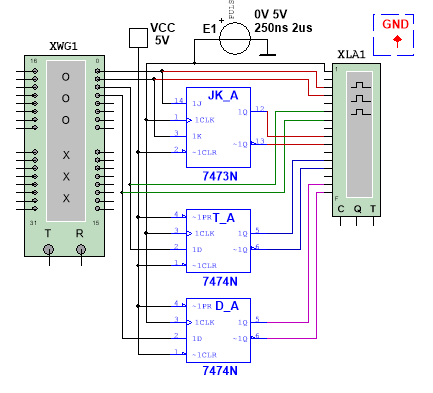
\includegraphics{trigger_scheme.png}}
	\caption{Схема для испытания триггеров \textit{JK, T} и \textit{D}.}
\end{figure}

\newpage

\textbf{Провести} моделирование работы триггеров в режимах \textbf{Step} или \textbf{Burst} генератора
\textbf{XWG1, скопировать} в отчет временные диаграммы, \textbf{составить} и \textbf{заполнить} таблицы
истинности работы триггеров \textbf{JK, T} и \textbf{D}. 

\begin{figure}[h]
	\center{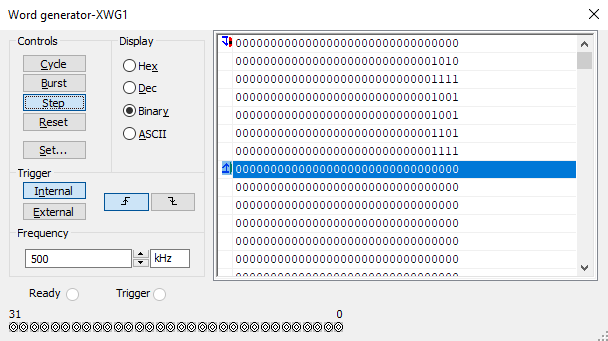
\includegraphics[scale=0.7]{word_set.png}}
	\caption{Набор кодовых комбинаций, соответствующих варианту 1.}
\end{figure}

\begin{figure}[h]
	\center{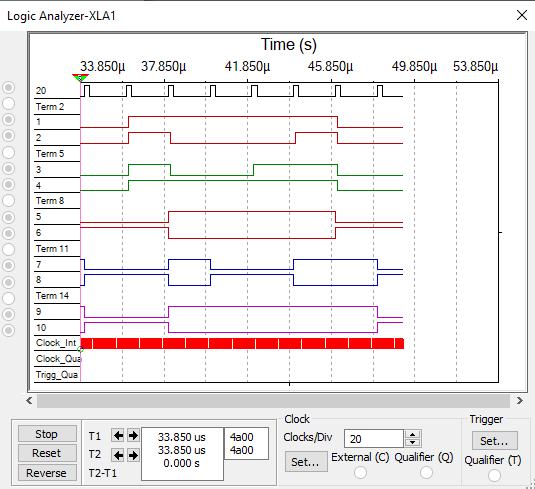
\includegraphics[scale=0.7]{logic_set.png}}
	\caption{Результат моделирования работы триггеров.}
\end{figure}

\newpage

\par Заполним таблицы истинности работы триггеров \textbf{JK, T} и \textbf{D}:

\begin{table}[h!]
    \centering
	\captionsetup{justification=centering}
	\begin{tabular}{|c|c|c|c|c|c|c|}
		\hline\xrowht[()]{10pt}
		$ SEQ_i $ & $ Q_{JK} $ & $ \overline{Q}_{JK} $ & $ Q_T $ & $ \overline{Q}_T $ & $ Q_D $ & $ \overline{Q}_D $ \\
        \hline\xrowht[()]{10pt}
          0000    &    0   &   1   &   0   &  1  &  0  &  1 \\
        \hline\xrowht[()]{10pt}
          1010    &    0   &   1   &   0   &  1  &  0  &  1 \\
        \hline\xrowht[()]{10pt}
          1111    &    1   &   0   &   1   &  0  &  1  &  0 \\
        \hline\xrowht[()]{10pt}
          1001    &    1   &   0   &   0   &  1  &  1  &  0 \\
        \hline\xrowht[()]{10pt}
          1001    &    1   &   0   &   0   &  1  &  1  &  0 \\
        \hline\xrowht[()]{10pt}
          1101    &    1   &   0   &   1   &  0  &  1  &  0 \\
        \hline\xrowht[()]{10pt}
          1100    &    0   &   1   &   1   &  0  &  1  &  0 \\
        \hline\xrowht[()]{10pt}
          0000    &    0   &   1   &   0   &  1  &  0  &  1 \\
        \hline
	\end{tabular}
	\caption{Таблица истинности работы триггеров \textit{JK, T, D} при заданных входных комбинациях.}
\end{table}

\newpage

\section*{Тестовые задания.}
\addcontentsline{toc}{section}{Тестовые задания}

\par 1. Укажите, какая \textbf{комбинация} логических сигналов является запрещенной для асинхронного RS-триггера: 
\textbf{11}.

\par 2. Укажите \textbf{условное графическое обозначение}:
\par a) \textit{JK}-триггера -- \textbf{г)};
\par б) \textit{RS}-триггера -- \textbf{в)};

\begin{figure}[h]
	\center{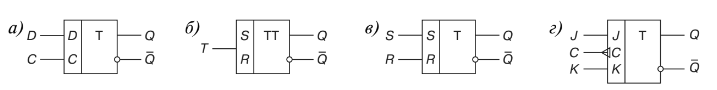
\includegraphics[scale=0.8]{triggers.png}}
\end{figure}

\par 3. Укажите \textbf{условное графическое обозначение}:

\par a) \textit{T}-триггера, выполненного на основе \textit{JK}-триггера -- \textbf{б)} (синхронный) и 
\textbf{д)} (асинхронный);
\par б) \textit{D}-триггера, выполненного на основе \textit{JK}-триггера -- \textbf{в)};

\begin{figure}[h]
	\center{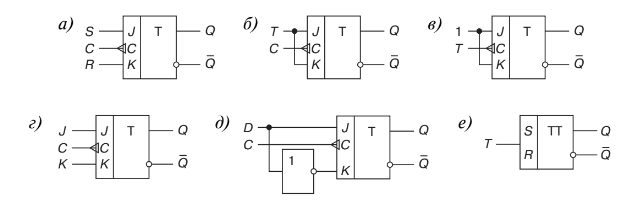
\includegraphics[scale=0.8]{based_triggers.png}}
\end{figure}

\par 4. Укажите, нашли ли широкое применение \textbf{асинхронные} \textit{D}-триггеры: триггер задержки 
(\textbf{D-триггер}) может быть только синхронным, так как имеет одининформационный \textit{D}-вход -- нет;

\par 5. Укажите, как \textbf{функционирует} \textit{JK}-триггер при комбинации \textit{J} = 1, 
\textit{К} = 1 на входе: одновременное присутствие логических единиц на информационных входах не является для 
\textit{JK}-триггера запрещенной комбинацией; при \textit{J} = 1 и \textit{K} = 1 \textbf{триггер работает в 
счетном режиме}, то есть переключается каждым тактовым импульсом на входе \textit{С};

\par 6. Укажите \textbf{время запаздывания} выходного сигнала по отношению к моменту подачи на \textit{С}-вход 
\textit{D}-триггера синхроимпульса при тактовой частоте $ f = 10 $ кГц ($ D^t = 1, Q^t = 0) $: 0,1 мс;

\par 7. Укажите значение \textbf{сигнала на выходе} \textit{JK}-триггера при комбинации \textit{J} = 1, 
\textit{К} = 0 на входе и \textit{Q} = 1 после окончания действия синхроимпульса: \textbf{1.};

\par 8. Укажите \textbf{аналитическое выражение}, описывающее работу:
\par a) \textit{RS}-триггера: $ Q^{t + 1} = S + Q^t \overline{R} $;
\par б) \textit{JK}-триггера: $ Q^{t + 1} = \overline{K}^t Q^t + J^t \overline{Q}^t $;
\par в) \textit{T}-триггера: $ Q^{t + 1} = Q^t \overline{T} + \overline{Q}^t T $;
\par г) \textit{D}-триггера: $ Q^{t + 1} = \overline{C}^t Q^t + C^t Q^t $;

\par 9. Укажите, чем отличается \textbf{динамическое управление} триггерами от статического управления: у 
триггеров с динамическим управлением сигналы на информационных входах должны оставаться неизменными на всем 
интервале действия активного логического сигнала синхронизации (\textit{С} = 1);

\par 10. Укажите \textbf{уровни напряжения} интегральных микросхем триггеров серии ТТЛ, принимаемые за логическую 
1 и логический 0 при напряжении питания $ U_n $ = 5 В: 2,4 В < $ U^1 $ < 5 В; 0 < $ U^0 $ < 0,4 В;

\par 11.Укажите, к какому \textbf{типу} триггеров относят Т-триггеры: \textbf{к синхронным.}

% Раздел "Заключение"
\conclusion

\par В ходе лабораторной работы мы ознакомились с основными характеристиками интегральных триггеров \textit{RS, D,
T} и \textit{JK} и испытали их на практике.

\newpage

%Библиографический список, составленный вручную, без использования BibTeX
%
%\begin{thebibliography}{99}
%  \bibitem{Ione} Источник 1.
%  \bibitem{Itwo} Источник 2
%\end{thebibliography}

%Библиографический список, составленный с помощью BibTeX
%
%\bibliographystyle{gost780uv}
%\bibliography{thesis}

% % При использовании biblatex вместо bibtex
%\printbibliography

% Окончание основного документа и начало приложений
% Каждая последующая секция документа будет являться приложением
\appendix

\end{document}